\chapter{Podstawy teorii muzyki i formatu MIDI} 
Zanim przejdziemy do omawiania poszczególnych części z jakich składa się utwór muzyczny. Należy wyjaśnić jedną zasadniczą kwestie - Muzyka istniała na tysiące lat zanim pojawiła się teoria ją opisująca.
Koncepcje i reguły składające się na teorie muzyki są w zasadzie podobne do reguł jakie stosuje się w języku naturalnym. Podobnie jak opanowanie gramatyki, pozwala na swobodne prowadzenie konwersacji, tak opanowanie reguł tworzenia muzyki pozwala lepiej tworzyć własne kompozycje i czytać cudze \citep[s. 22]{Pilhofer2018}.

Wiele osób uważa, że teoria muzyki powstała w starożytnej Grecji, ale pierwsze instrumenty muzyczne, zdaniem historyków, powstały już około 7000 lat p.n.e. W okresie formowania się pierwszych osad ludzkich, na długo przed Starożytną Grecją. Na niektórych replikach fletów z kości słoniowej, które powstały w tamtym okresie nadal da się tworzyć utwory muzyczne. Fakt ten nie umniejsza oczywiście osiągnięciom Greków - Pitagoras z Samos stworzył dwunastodźwiękową przypominająca tą, której muzycy używają współcześnie. Stworzył także pierwsze \textit{koło kwintowe}.\footnote{Jest to rodzaj schematów pozwalający opisać pokrewne tonacje poszczególnych dźwięków.} W istocie wkład starożytnych Greków w muzykę był na tyle znaczny, że przez dłuższy czas nie wprowadzano do niej żadnych znacznych modyfikacji \citep[s. 23]{Pilhofer2018}.

\section{Podstawy teorii muzyki} 
Wyjaśnienie podstaw teorii muzyki zaczniemy od jej części składowych: \textit{nut, pauz i tempa}.
Tempo (bit) to pulsacja dzieląca czas na równe odcinki. To czym jest bit dobrze uosabia mechanizm działania zegara. Na każdą minutę składa się 60 tyknięć wskazówki sekund, a każde z tych tyknięć to oddzielny bit. Jeśli przyspieszymy lub spowolnimy wskazówkę zegara, to zmienimy \textit{tempo} tyknięć. Rolą nut w muzyce jest przekazywanie informacji o tym co powinno być zagrane w każdej z oddzielnych tyknięć. Innymi słowy mówią one o tym jak długo i jak często powinno się zagrać określoną \textit{wysokość dźwięku} \citep[s. 31]{Pilhofer2018}.

Każda nuta ma budowę trzyczęściową. Składa się z \textit{główki, ogonka} i \textit{chorągiewki}.
\begin{itemize}
 \item Główka to okrągła część nuty, każda nuta ją ma. Cała nuta składa się tylko z główki,
 \item Ogonek to pionowa linia wychodząca od główki. Mają ją \textit{ósemki, ćwierćnuty} i \textit{półnuty},
 \item Chorągiewka to mała linia wychodząca z lub od ogonka. Chorągiewkę ma \textit{ósemka} i każda nuta od niej krótsza \citep[s. 32-33]{Pilhofer2018} (zob. rys. 3.1).
\end{itemize}

\begin{figure}[H]
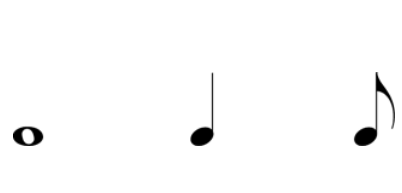
\includegraphics[scale = 0.8]{nuty.png}
\centering
\caption{Od lewej: cała nuta, ćwierćnuta i ósemka. Źródło: \citep[s. 33]{Pilhofer2018}.}
\centering
\end{figure}

Zamiast rysować chorągiewkę przy każdej nucie, można je połączyć \textit{belką}, która trochę upraszcza zapis. (zob. rys. 3.2).

\begin{figure}[H]
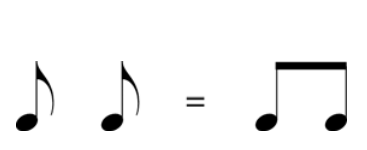
\includegraphics[scale = 0.7]{belka.png}
\centering
\caption{Ósemki można zapisywać oddzielnie lub razem łącząc je za pomocą belki. Źródło: \citep[s. 33]{Pilhofer2018}.}
\centering
\end{figure}
Kolejny rysunek przedstawia szesnastki z chorągiewkami. Sposób zapisu nie ma znaczenia, gdyż wszystkie gra się tak samo (zob. rys. 3.3).
\begin{figure}[H]
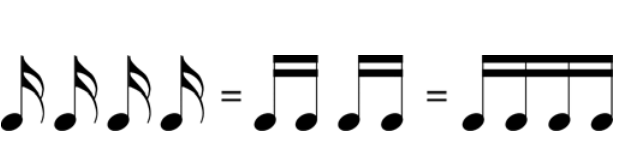
\includegraphics[scale = 0.7]{szesnastki.png}
\centering
\caption{Szesnastki pogrupowane jako: pojedyncze nuty, szesnastki połączone podwójnymi belkami oraz jako grupę nut połączonych jedną podwójną belką. Źródło: \citep[s. 33]{Pilhofer2018}.}
\centering
\end{figure}

Dobrym sposobem na prześledzenie w jaki sposób rozkładają się wartości poszczególnych nut jest skorzystanie z \textit{drzewa nut} pokazanego na rysunku 3.4. 

\begin{figure}[H]
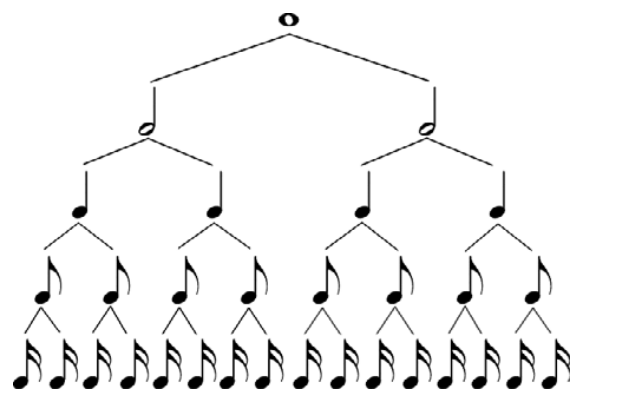
\includegraphics[scale = 0.8]{drzewo.png}
\centering
\caption{Drzewo nut składa się z całej nuty rozkładającej się na dwie półnuty, które następnie rozkładają się na cztery ćwierćnuty. Ćwierć nuty rozkładają się na ósemki, a ósemki na szesnastki Źródło: \citep[s. 34]{Pilhofer2018}.}
\centering
\end{figure}

\textit{Pauza} to cisza w muzyce. Pauzy są szczególnie ważne gdy piszę się utwory, które mają być czytane przez innych ludzi. Pozwalają one na precyzyjniejsze wskazanie rytmu niż za pomocą samych nut. Rysunek 3.5 przedstawia względne wartości pauz. Podobnie jak w drzewie nut na samej górze jest pauza całonutowa, potem półnutowa, ćwierćnutowa, ósemkowa i szesnastkowa \citep[s. 40-41]{Pilhofer2018}

\begin{figure}[H]
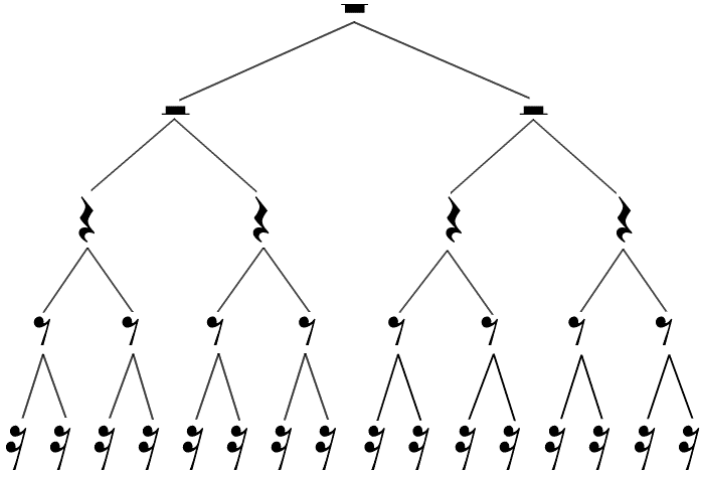
\includegraphics[scale = 0.7]{pauzy.png}
\centering
\caption{Drzewo pauz. Źródło: \citep[s. 42]{Pilhofer2018}.}
\centering
\end{figure}

Nuty i pauzy zapisuje się na \textit{pięciolinii} (zob. rys. 3.6). Pięciolinia składa się z pięciu równoległych poziomych linii i czterech przerw między liniami. Nuty i pauzy umieszczane są na liniach, jak i na przerwach między liniami. Wysokość dźwięku oznaczana przez poszczególne linie i przerwy jest wskazywana przez \textit{klucz} znajdujący się na początku pięciolinii. Istnieją dwa główne rodzaje kluczy:
\begin{enumerate}
    \item klucz wiolinowy -- za jego pomocą oznacza się pięciolinie do zapisu wyższych dźwięków,
    \item klucz basowy -- tego rodzaju pięciolinii używa się do grania niższych dźwięków,
\end{enumerate}

Pięciolinia umożliwia wygodne przedstawienie wysokości dźwięku (zarówno pojedynczo jak i w akordach), z uwzględnieniem czasu ich trwania.
 Każda wysokość lub ton na pięciolinii ma nazwę jednej z siedmiu liter alfabetu: \textit{A,H,C,D,E,F,G,A,H,C}.
 
 \begin{figure}[H]
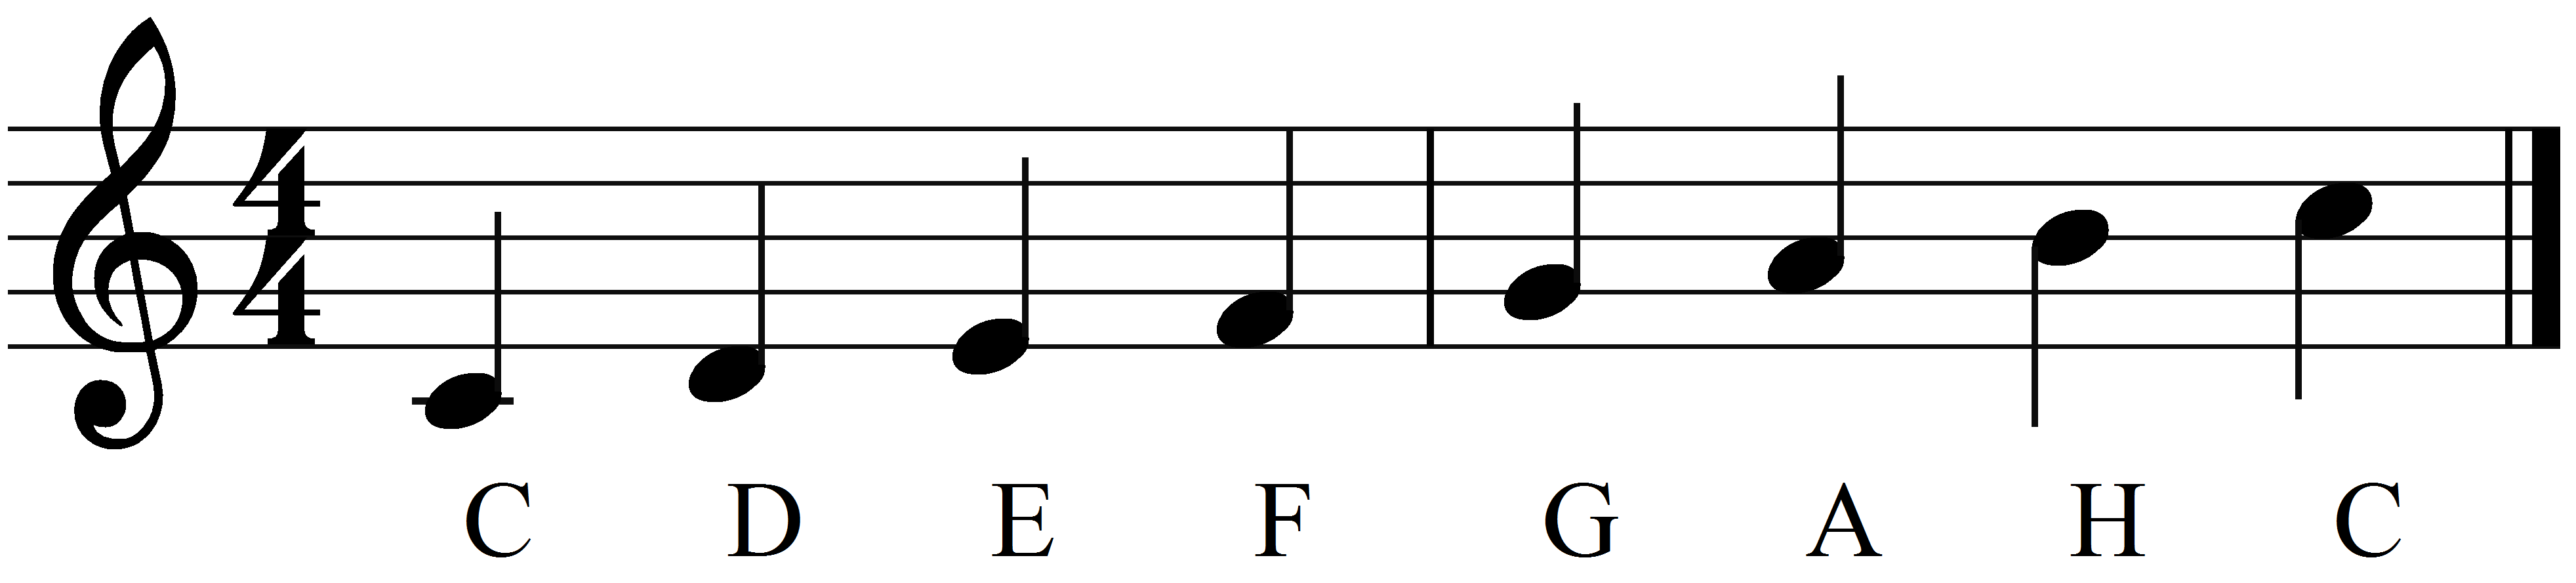
\includegraphics[scale = 0.8]{pieciolinia.png}
\centering
\caption{Gama C-dur. C-dur to tonacja muzyczna oparta na skali durowej. Zawiera siedem dźwięków od A do H(B). Źródło: https://pl.wikipedia.org/wiki/C-dur}
\centering
\end{figure}

Jeśli teoria muzyki to wiedza na temat tego z jakich elementów można stworzyć muzykę, to \textit{kompozycją} nazywamy umiejętność budowania \textit{utworu muzycznego} z tych podstawowych elementów \citep[s. 22]{Usarzewicz2018}.
Poza nutami, tempem i pauzą. Utwór muzyczny składa się także z \textit{interwałów}, \textit{akordów} oraz \textit{skal}.

\textit{Interwał} to inaczej odległość pionowa między dwoma dźwiękami na pięciolinii (zob. rys. 3.7) 

 \begin{figure}[H]
 \centering
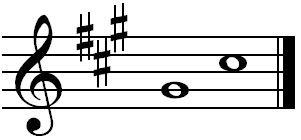
\includegraphics[scale= 0.4]{interwal.png}
\caption{Interwał. Źródło: \citep[s. 22]{Usarzewicz2018}.}
\centering
\end{figure}

\textit{Akord} to współbrzmienie co najmniej trzech dźwięków ułożonych na pięciolinii jeden nad drugim. Akordy są ważnym elementem budującym \textit{harmonie} w utworze. Harmonia zajmuje się łączeniem akordów w większe całości (zob. rys. 3.8) \citep[s. 23]{Usarzewicz2018}.

 \begin{figure}[H]
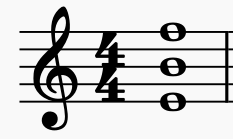
\includegraphics[scale = 0.7]{akord.png}
\centering
\caption{Akord. Źródło: Opracowanie własne w programie MuseScore.}
\centering
\end{figure}

Zestaw następujących po sobie dźwięków, ułożonych w określonej kolejności, to \textit{skala muzyczna}. Najczęściej spotyka się skale \textit{minorową(molową)} i \textit{majorową(durową)} Utwory oparte na skali molowej często uważa się za mające smutne brzmienie. Natomiast utwory oparte o skale durową często uważa się za radosne. Na rysunku 3.9 przedstawiono jedną ze skal tak zwaną \textit{pentatonikę} \citep[s. 81 - 82]{Pilhofer2018}. 

 \begin{figure}[H]
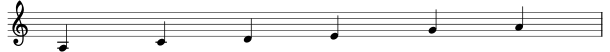
\includegraphics[width=\textwidth]{pentatonika.png}
\caption{Pentatonika z dźwiękiem centralnym D. Pentatonika to jedna z tradycyjnych skal muzycznych, która wywodzi się ze starożytności i jest popularna w muzyce ludowej  Źródło: https://pl.wikipedia.org/wiki/Pentatonika}
\centering
\end{figure}

\section{Format MIDI}
\textit{MIDI} to z języka angielskiego \textit{cyfrowy interfejs instrumentów muzycznych}. Służy on do przekazywania informacji pomiędzy cyfrowymi instrumentami muzycznymi. MIDI umożliwia komputerom, syntezatorom, keyboardom i kartom dźwiękowym komunikowanie się w wspólnym standardzie wymiany informacji oraz pozwala synchronizować się nawzajem. System ten pozwolił także na stworzenie łatwych w obsłudze \textit{sekwencerów} i \textit{syntezatorów perkusyjnych}.

Standard MIDI został stworzony w roku 1983 i znacznie ułatwił pracę z syntezatorami dźwięku. W czasach przed MIDI każdy syntezatorów należało indywidualnie zaprogramować \citep{MIDI}.

W przeciwieństwie do innych formatów audio (jak .flac lub .wav) format MIDI sam w sobie nie przechowuje dźwięku, zawiera jedynie instrukcje jak dany dźwięk zrekonstruować, Jest swoistym rodzajem \textit{cyfrowej pięciolinii} \citep[s. 1 - 2]{MIDI_Format}.
Protokół MIDI pozwala na wysłanie informacji przez maksymalnie 16 różnych kanałów, co pozwala na jednoczesną grę do 16 różnych instrumentów. Można powiedzieć, że standard MIDI specyfikuje zarówno wymagania wstępne względem typu urządzenia mającego odtwarzać dźwięk jak i sam protokół transmisji, podług którego mają być wysyłane wiadomości w standardzie MIDI. Struktura pliku MIDI została pokazana na rysunku 3.10 \citep[s. 1 - 2]{MIDI_Format}.

\begin{figure}[H]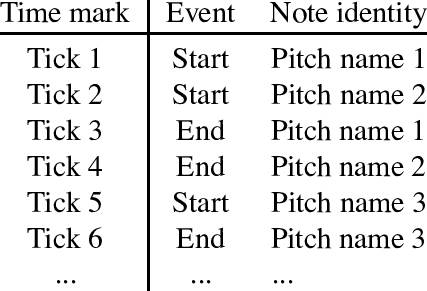
\includegraphics[scale=0.6]{MIDI_file.png}
\centering
\caption{Struktura pliku MIDI. Plik MIDI składa się z tzw. \textit{eventów}, które zawierają informacje o treści wiadomości MIDI oraz o czasie jej nadania. Źródło: \citep[s. 2 - 3]{MIDI_Format} i \citep{Tse2008}.}
\end{figure}

Aby skorzystać z możliwości jakie daje nam MIDI należy zaopatrzyć się w instrumenty. Instrumenty mogą być dystrybuowane niezależnie jako pakiety \textit{VSTi} dołączane oddzielnie do \textit{syntezatora programowego} takiego jak \textit{Helm} (zob. rys. 3.11)
Do tworzenia muzyki w formacie MIDI można wykorzystać także \textit{syntezator sprzętowy} taki jak \textit{klawiatura MIDI} Klawiatura jest rodzajem kontrolera wysyłającego sygnały elektryczne w formacie MIDI, które sam protokół interpretuje i odtwarza jako dźwięk. Przykład takiej klawiatury to rysunek 3.12. warto zwrócić uwagę na to, że każdej nucie na klawiaturze przyporządkowany jest odpowiadający mu numer kodu formatu MIDI.

\begin{figure}[H]
\centering
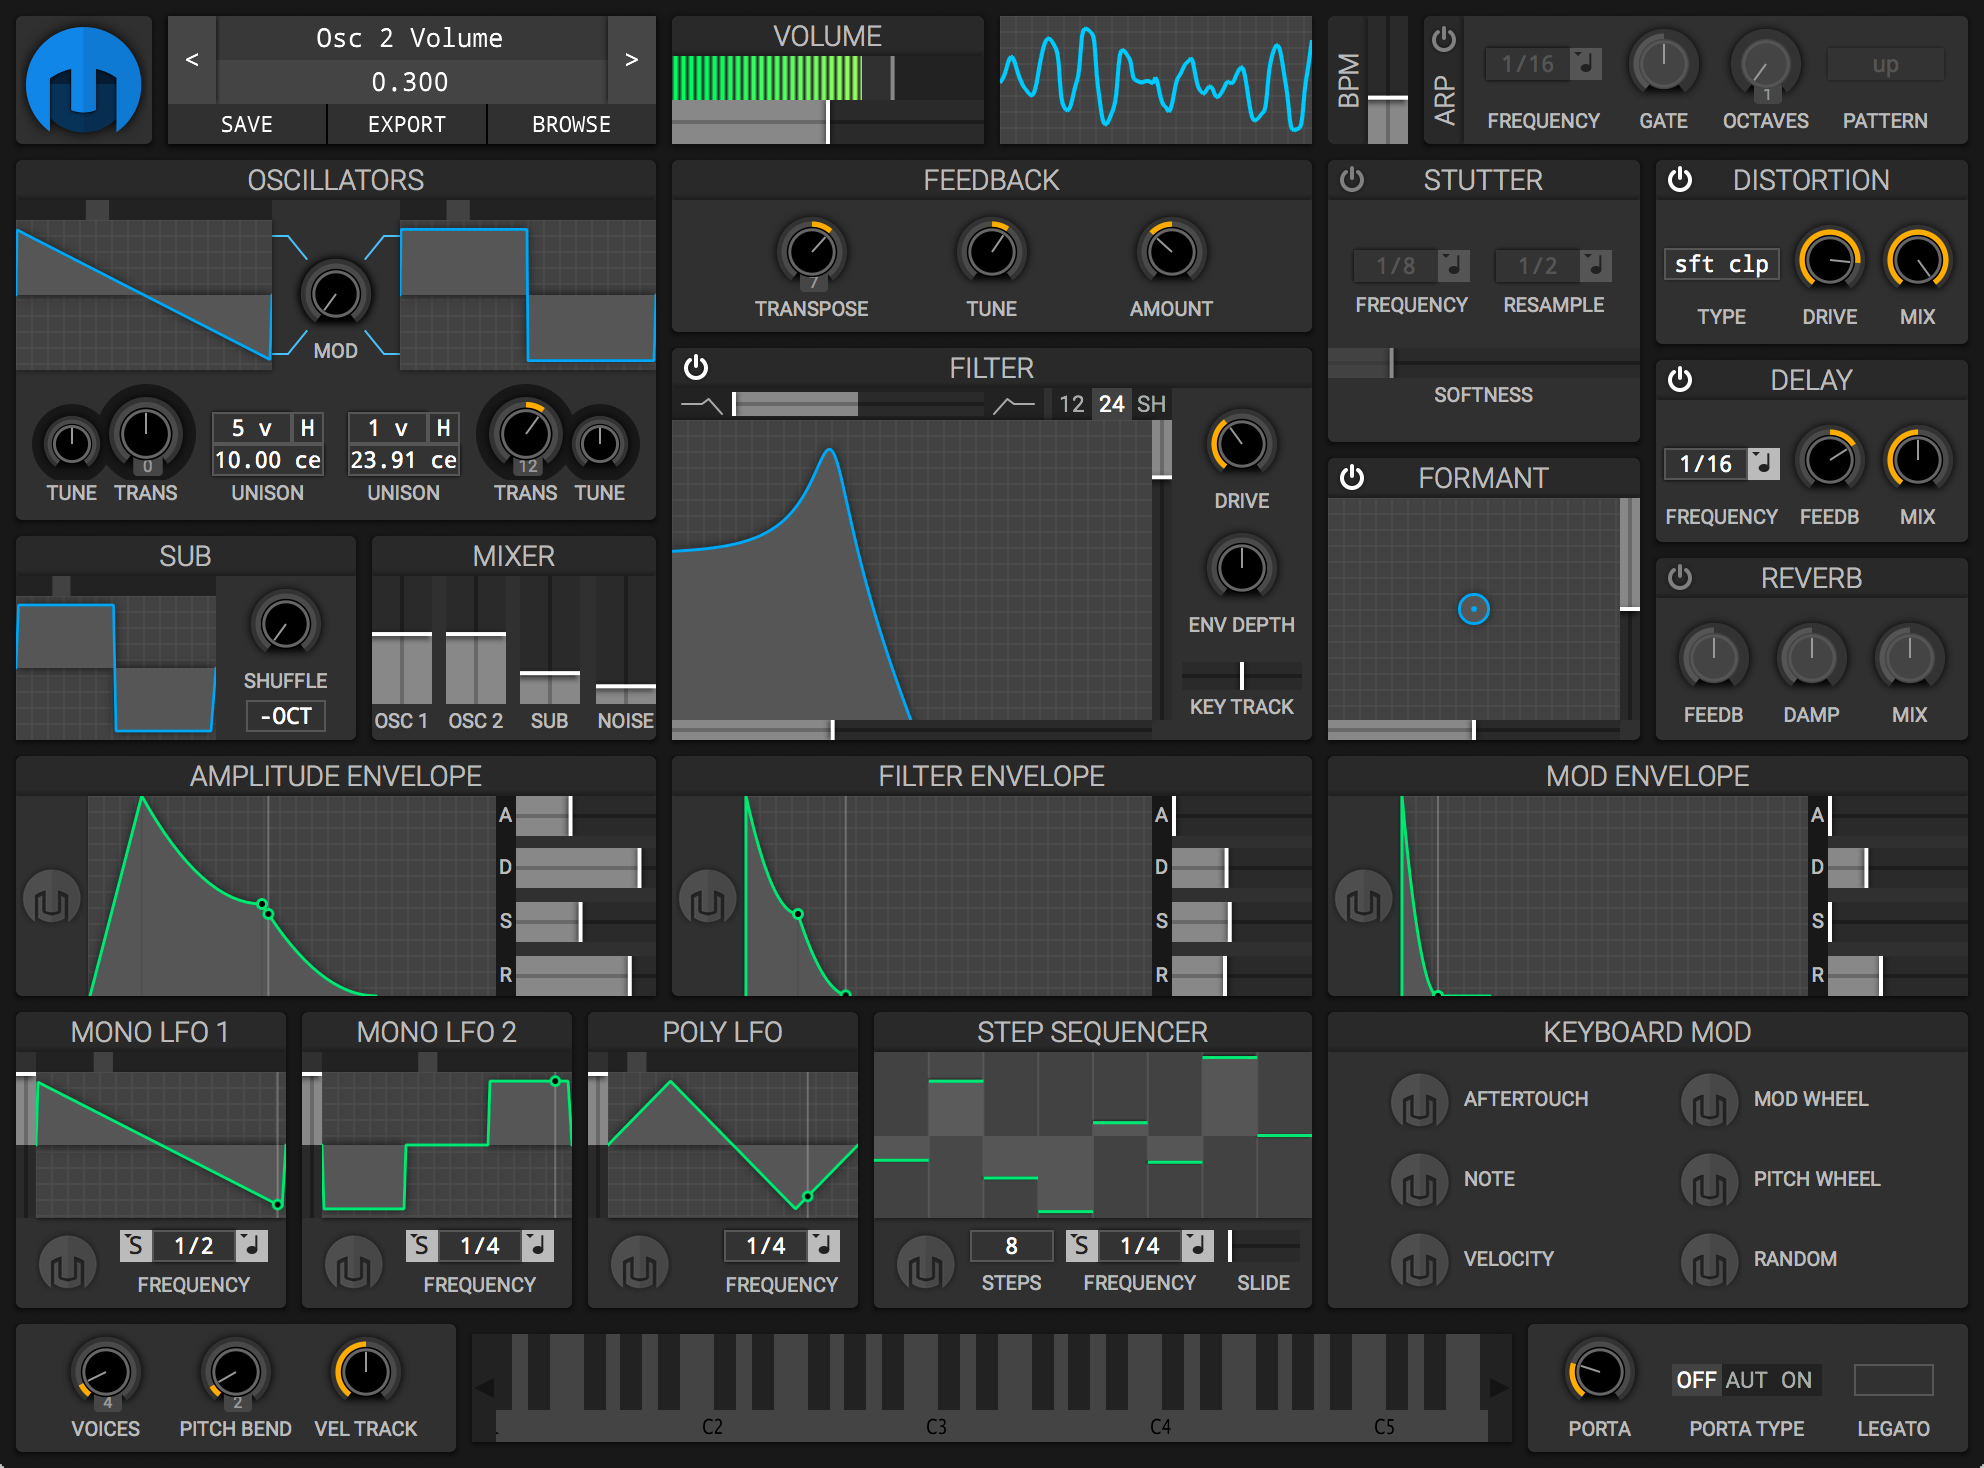
\includegraphics[scale = 0.35]{helm.png}
\centering
\caption{Interfejs programu Helm. Źródło: https://tytel.org/helm/}
\end{figure}


\begin{figure}[H]
\begin{center}
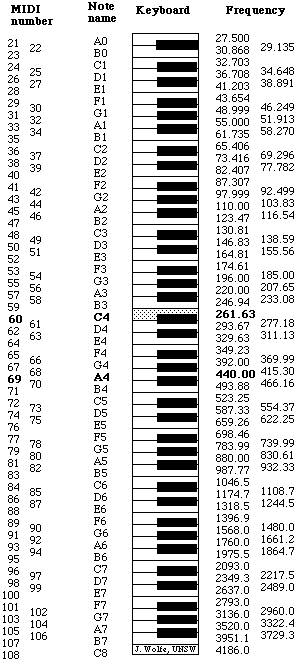
\includegraphics[scale = 0.8]{midi.png}
\centering
\caption{Klawiatura MIDI, Źródło: \href{https://pl.wikipedia.org/wiki/MIDI}{https://pl.wikipedia.org/wiki/MIDI}}
\centering
\end{center}
\end{figure}
 
